\item
The given equations can be expressed as the matrix equation
\begin{align}
\myvec{1 & -3\\3 & -9} \vec{x} = \myvec{3\\2}
\end{align}
%
The augmented matrix for the above equation is row reduced as follows
\begin{align}
\myvec{1 & -3 & 3\\3 & -9 & 2} 
\xleftrightarrow {R_2\leftarrow R_2 -3R_1}\myvec{1 & \ -3 & 3 \\0 & 0 & -7 }
\end{align}
%
$\therefore$ the lines in \eqref{linform/11/ab/1.0.1} are parallel as can be seen in Fig. \ref{linform/11/ab/figure: parallel lines.}.
%
\begin{figure}[ht!]
\centering
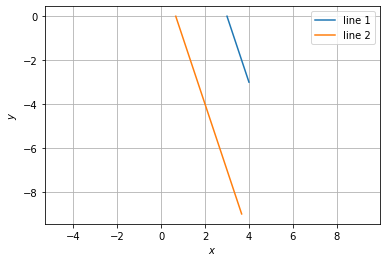
\includegraphics[width=\columnwidth]{solutions/su2021/2/11/ab/Parallel_ lines (1).png}
\caption{PARALLEL LINES.}
\label{linform/11/ab/figure: parallel lines.}
\end{figure}
\item
The given  equations can be expressed as the matrix equation
\begin{align}
\myvec{2 & 1\\3 & 2}
\vec{x} = \myvec{5\\8}
\end{align}
%
The augmented matrix for the above equation is row reduced as follows
\begin{align}
\myvec{2 & 1 & 5\\3 & 2 & 8 }
\xleftrightarrow {R_2\leftarrow 2R_2-3R_1}\myvec{2 & 1 &5 \\0 & 1 & 1}
\\
\myvec{2 & 1 & 5\\0 & 1 & 1}
\xleftrightarrow {R_1\leftarrow
R_1-R_2}\myvec{2 & 0 & 4\\0 & 1 & 1}
\\
\myvec{2 & 0 & 4\\0 & 1 & 1}
\xleftrightarrow{R_1\leftarrow \frac{R_1}{2}}\myvec{1 & 0 & 2\\0 & 1 & 1}
\end{align}
Thus, 
\begin{align}
\vec{x}&= \myvec{2 \\ 1}
\end{align} is the point of intersection of the lines in 
\eqref{linform/11/ab/1.0.2} as verified in Fig.     \ref{linform/11/ab/fig: INTERSECTING LINES.}.
%
\begin{figure}[ht]
    \centering
   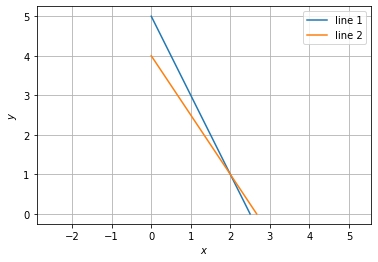
\includegraphics[width=\columnwidth]{solutions/su2021/2/11/ab/Intersecting lines .png}
    \caption{INTERSECTING LINES.}
    \label{linform/11/ab/fig: INTERSECTING LINES.}
\end{figure}    

